\documentclass[times, utf8, zavrsni]{fer}
\usepackage{booktabs}
\usepackage{graphicx}
\usepackage[]{algorithm2e}
\usepackage{caption}
\graphicspath{{/home/mateo/Git/Kraken_memory_improvement/Pictures/}}
\begin{document}
\captionsetup[algorithm2e]{name=Algoritam}
% TODO: Navedite broj rada.
\thesisnumber{5133}

% TODO: Navedite naslov rada.
\title{Algoritam staničenja velike baze podataka genoma}

% TODO: Navedite vaše ime i prezime.
\author{Mateo Stjepanović}

\maketitle

% Ispis stranice s napomenom o umetanju izvornika rada. Uklonite naredbu \izvornik ako želite izbaciti tu stranicu.
\izvornik

% Dodavanje zahvale ili prazne stranice. Ako ne želite dodati zahvalu, naredbu ostavite radi prazne stranice.
\zahvala{Zahvaljujem mentorici doc.\ dr.\ sc.\ Mirjana Domazet-Lošo na podršci.}

\tableofcontents

\chapter{Uvod}
Bioinformatika je interdisciplinarna znanost koja se bavi razvojem programa i metoda za interpretiranje bioloških podataka. Spaja matematiku, statistiku, računalnu znanost te druge prirodno matematičke znanosti. U posljednjem desetljeću bioinformatika kao znanost doživaljava veliki porast, te kao takva uspjeva mapirati genome mnogih živih bića.\\
U navedenom porastu najviše se ističu metode analiziranja genoma, te, spajanjem statističkih analiza i algoritama iz područja računalne znanosti, metode određivanja položaja istih u taksonomskom stablu. Upravo u tom području postoje mnogi alati koji su razvijeni upravo s ciljem poboljšanja točnosti određivanja taksonomskog stabla novoj, nepoznatoj, jedinki.\\ Za većinu jedinki u uzorku su vrsta, rod i više razine stabla nepoznati. Ako je jedinka potpuno nepoznata tada će se klasificirati kao nova nepoznata vrsta te se neće dalje klasificirati. U velikom broju slučajeva će postojati neke sličnosti sa nekim već određenim vrstama, te je potrebno pronaći te sličnosti kako bi se sjedinka uspješno klasificirala. Za to služe razni algoritmi poravnanja. Jedan od tih je BLAST. Postoje druge metode i programi koji pospješuju učinkovitost BLAST-a uvođenjem metoda strojnog učenja. Iako bolje preciznosti ti programi imaju jednu veliku manu. Vrijeme potrebno za klasificiranje podatka je jako veliko, stoga su više manje neiskoristivi. \\Tu na scenu nastupa alat za klasifikaciju metagenoma nazvan Kraken(Derrick E. Wood i Steven L.).
\\{\textit{Kraken is ultrafast and high accurate program for assigning taxonomic labels to metagenomic DNA sequences.}\footnote[1]{Wood and Salzberg: \textbf{Kraken: ultrafast metagenomic sequence classification using exact alignments.} \textit{Genome Biology} 2914 15:R46}
\\Za razliku od alata koji su pokušali poboljšati preciznost BLAST algoritma, te time izgubili na brzini, Kraken je jedan od rijetkih alata koji postiže točnost koja premašuje onu u BLAST algoritmu, s time da ne gubi na brzini izvođenja. Rad Krakena se sastoji od toga da se ulazni podatak "razbija" na k-mere, te se minimizer algoritmom traže oni k-meri koji imaju istu vrijednost minimzer-a. Tada se taj podatak uspoređuje s podacima u Kraken-ovoj bazi podataka, s tim da je baza sortirana na način da su podaci sa istim minimizerom smješteni jedan pored drugog, tako da se pretraživanje jako pospješuje i ubrzava. Autori alata su shvatili da Kraken može naići an problem prilikom izvođenja na računalu s ograničenim resursima, točnije na računalu s RAM-om ispod 70GB. Iz tog razloga je razvijena MiniKraken baza podataka koja je sa prvotnih 70GB podataka smanjena na 4GB.
\begin{table}[htb]
	\centering
	\resizebox{\textwidth}{!}{%
		\begin{tabular}{|llcccccc|}
			\hline
			\multicolumn{1}{|c}{} & \multicolumn{1}{c}{}  & \multicolumn{2}{c}{HiSeq}                                       & \multicolumn{2}{c}{MiSeq}                                       & \multicolumn{2}{c|}{simBA-5}                                     \\
			\multicolumn{2}{|l}{Classifier}              & \multicolumn{1}{l}{Precision} & \multicolumn{1}{l}{Sensitivity} & \multicolumn{1}{l}{Precision} & \multicolumn{1}{l}{Sensitivity} & \multicolumn{1}{l}{Precision} & \multicolumn{1}{l|}{Sensitivity} \\ \hline
			Megablast             & \multicolumn{1}{l|}{} & \multicolumn{1}{c|}{99.03}    & \multicolumn{1}{c|}{79.00}      & \multicolumn{1}{c|}{92.44}    & \multicolumn{1}{c|}{75.76}      & \multicolumn{1}{c|}{96.93}    & 93.67                            \\ \hline
			NBC                   & \multicolumn{1}{l|}{} & \multicolumn{1}{c|}{82.33}    & \multicolumn{1}{c|}{82.33}      & \multicolumn{1}{c|}{77.78}    & \multicolumn{1}{c|}{77.78}      & \multicolumn{1}{c|}{97.64}    & 97.64                            \\ \hline
			PhymmBL               & \multicolumn{1}{l|}{} & \multicolumn{1}{c|}{79.14}    & \multicolumn{1}{c|}{79.14}      & \multicolumn{1}{c|}{76.21}    & \multicolumn{1}{c|}{76.21}      & \multicolumn{1}{c|}{96.11}    & 96.11                            \\ \hline
			PhymmBL65             & \multicolumn{1}{l|}{} & \multicolumn{1}{c|}{99.13}    & \multicolumn{1}{c|}{73.95}      & \multicolumn{1}{c|}{92.47}    & \multicolumn{1}{c|}{73.03}      & \multicolumn{1}{c|}{99.08}    & 95.45                            \\ \hline
			Kraken                & \multicolumn{1}{l|}{} & \multicolumn{1}{c|}{99.20}    & \multicolumn{1}{c|}{77.15}      & \multicolumn{1}{c|}{94.71}    & \multicolumn{1}{c|}{73.46}      & \multicolumn{1}{c|}{99.90}    & 91.25                            \\ \hline
			Kraken-Q              & \multicolumn{1}{l|}{} & \multicolumn{1}{c|}{99.12}    & \multicolumn{1}{c|}{76.31}      & \multicolumn{1}{c|}{94.69}    & \multicolumn{1}{c|}{70.41}      & \multicolumn{1}{c|}{99.92}    & 89.54                            \\ \hline
			MiniKraken            & \multicolumn{1}{l|}{} & \multicolumn{1}{c|}{99.44}    & \multicolumn{1}{c|}{66.12}      & \multicolumn{1}{c|}{97.41}    & \multicolumn{1}{c|}{67.95}      & \multicolumn{1}{c|}{99.95}    & 65.87                            \\ \hline
			MiniKraken-Q          & \multicolumn{1}{l|}{} & \multicolumn{1}{c|}{99.36}    & \multicolumn{1}{c|}{65.67}      & \multicolumn{1}{c|}{97.32}    & \multicolumn{1}{c|}{65.84}      & \multicolumn{1}{c|}{99.98}    & 65.31                            \\ \hline
			Kraken-GB             & \multicolumn{1}{l|}{} & \multicolumn{1}{c|}{99.51}    & \multicolumn{1}{c|}{93.75}      & \multicolumn{1}{c|}{98.48}    & \multicolumn{1}{c|}{86.23}      & \multicolumn{1}{c|}{99.48}    & 91.13                            \\ \hline
		\end{tabular}%
	}
	\caption{Klasifikacija roda za tri metagenoma}
	\label{StatRez}
\end{table}


\chapter{Definiranje problema}
Uz već spomenutost rješenja problema korištenja velike količine resursa, nailazi se na problem koji će se pokušati riješiti tijekom ovog rada.
% Please add the following required packages to your document preamble:
% \usepackage{graphicx}
\begin{table}[hbp]
	\centering
	\resizebox{\textwidth}{!}{%
		\begin{tabular}{|llcccccc|}
			\hline
			\multicolumn{1}{|c}{} & \multicolumn{1}{c}{} & \multicolumn{2}{c}{HiSeq} & \multicolumn{2}{c}{MiSeq} & \multicolumn{2}{c|}{simBA-5} \\
			\multicolumn{2}{|l}{Classifier} & \multicolumn{1}{l}{Precision} & \multicolumn{1}{l}{Sensitivity} & \multicolumn{1}{l}{Precision} & \multicolumn{1}{l}{Sensitivity} & \multicolumn{1}{l}{Precision} & \multicolumn{1}{l|}{Sensitivity} \\ \hline
			Kraken & \multicolumn{1}{l|}{} & \multicolumn{1}{c|}{99.20} & \multicolumn{1}{c|}{77.15} & \multicolumn{1}{c|}{94.71} & \multicolumn{1}{c|}{73.46} & \multicolumn{1}{c|}{99.90} & 91.25 \\ \hline
			MiniKraken & \multicolumn{1}{l|}{} & \multicolumn{1}{c|}{99.44} & \multicolumn{1}{c|}{66.12} & \multicolumn{1}{c|}{97.41} & \multicolumn{1}{c|}{67.95} & \multicolumn{1}{c|}{99.95} & 65.87 \\ \hline
		\end{tabular}%
	}
	\caption{Isječak iz Tablice 1.1}
	\label{IsjecakTablice}
\end{table}

Iako se iz dane tablice vidi da se preciznost korištenjem MiniKraken baze podataka neznatno povećala u odnosu na Kraken bazu podataka. S druge strane osjetljivost jako opada. Osjetljivost predstavlja mjeru koja određuje postotak uočenih lažno negativnig podataka, tj. predstavlja postotak točno kvalificiranih podataka koji su uistinu tako i predstavljeni. S druge strane precizonst predstavlja izbjegavanje lažno pozitivnih podataka, tj. koliko podataka je uočeno da ne pripadaju nekoj skupini, s tim da oni uistinu ne pripadaju toj skupini.\\Ideja ovog rada je da se algoritmima sličnim algoritmima straničenja osposobi računalo s ograničenim resursima za rad s bazom podataka čija veličina uvelike nadilazi količinu RAM-a raspoloživog na računalu. Prvotno je potrebno podjeliti bazu podataka na više manjih koje će se moći uspješno učitati u memoriju te pretražiti. Ideja je iskoristiti "kontejnere" k-mera koji su određeni svaki jedinstvenom minimizer vrijednosti, te pomoću binarnog pretraživanja indeksa učitavati samo onu bazu podataka pomoću koje je moguće klasificirati podatak u taksonomsko stablo. Želeći se približit straničenju, predstavit će se samo iteriranje po indeksima te učitavati slijedno baze podataka i pretraživati svaku.
\chapter{Strukture podataka i algoritmi u Kraken-u}
\subsection{Baza podataka}
\subsubsection{Kreiranje baze podataka}

Nastanak baze podataka se događa u nekoliko koraka. Za početak se sa NCBI-a preuzimaju biblioteke koje sadrže trenutno poznate vrste. Budući da pretraživanje baze podataka u Kraken-u osniva na k-merima potrebno je proizvesti k-mere za svaki podataka u bazi podataka. Za to služi alat naziva Jellyfish(Guillaume Marçais i Carl Kingsford) koji računa k-mere zadane duljine 31 ( korisnik također može zadati duljinu k-mera).\\Jellyfish je alat za brzo i memorijski povoljno prebrojavanje podnizova u danom nizu. Za potrebe prilagodbe svim resursima za Jellyfish postoje opcije za brzo izračunavanje koje je memorijski zahtjevnije, te ono sporije ali memorijski ne toliko zahtjevno. U kontekstu bioinformatike Jellyfish se koristi za prebrojavanje k-mera u zadanom metagenomu. Sam rad se bazira na hash tablici koja je osposobljena za paralelan rad preko više CPU-a. Hash tablica se sastoji od para (ključ,vrijednost), gdje je ključ zadani k-mer a vrijednost je broj njegovog ponavljanja u metagenomu.
	 	
\begin{table}[hbp]
	\centering
	\caption{Prikaz niza te njegovih k-mera (k = 4)}
	\label{Prikaz k-mera}
	\begin{tabular}{llllllllll}
		Ulaz:  &           & \multicolumn{8}{l}{AGATCGAGTG}                            \\
		4-mer: & \multicolumn{2}{l}{} & AGAT & GATC & ATCG & TCGA & CGAG & GAGT & AGTG
	\end{tabular}
\end{table}
Nakon rada Jellyfish-a u bazu se spremaju 4 bajtne vrijednosti k-mera te se kreira identifikacijska oznaka za svaki podataka. Tada program kreiranja baze podataka ponovno prolazi kroz istu, te za svaki identifikator podatka izračunava njegov LCA(\textit{Najmanji zajednički predal}), te ga sprema u bazu podataka zajedno s identifikatorom i njegovim k-merima.
\subsubsection{Strukture baze podataka}
Gore navedeni proces klasificiranja ulaznog genoma pomoću baze podataka se , već navedeno, bazira na pretraživanju k-mera. Baza podataka se sastaoji od identifikacijskih oznaka svakog podatka u njoj, njihovog izračunatog najmanjeg zajedničkog pretka, te k-mera koje on tvori.\\
\begin{figure}[hbp]
	\centering
	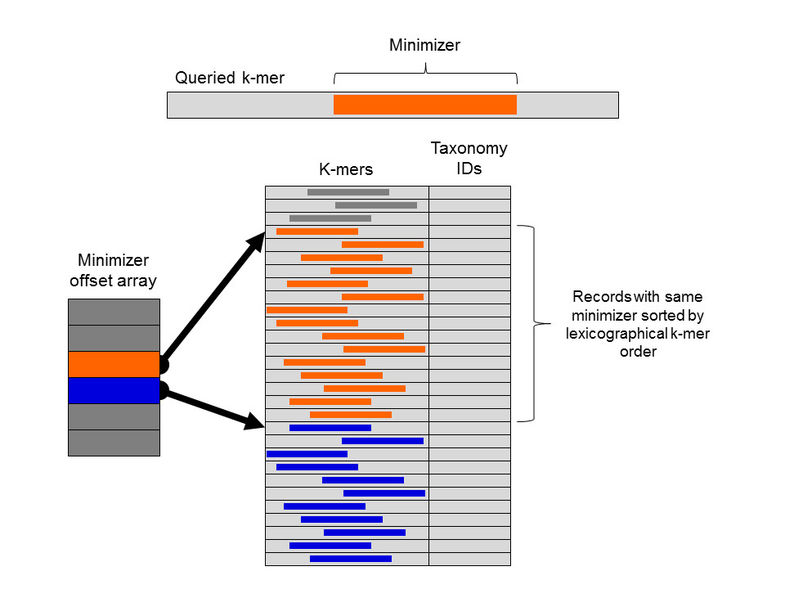
\includegraphics[width=\textwidth]{DbStructure.jpg}
	\caption{Prikaze strukture baze podataka}
	\label{BazaPodataka}
\end{figure}

S ciljem poboljšanja brzine pretraživanja, uvodi se algoritam indeksiranja i raspoređivanja poznat pod imenom Minimizer (Roberts M, Hayes W, Hunt B, Mount s, te Yorke J.).
 

\begin{algorithm}[H]
	\SetAlgorithmName{Algoritam}{algoritam}{List of algoritam}
	ptr <- pokazivač\_na\_k-mer\;
	k\_ct <- brojač kontejnera\;
	vrijednosti <- 1ull << (nt * 2);
	\While{brojač je različit od broja kontejnera}{
		brojač++\;
		dohvati\_k-mer(ptr)\;
		ključ <- izračunaj\_ključ()\;
		b\_brojac[ključ]++\;		
	}
	b\_ofset\_ofset[vrijednosti +1]\;
	\For{i < vrijednosti}{
		b\_ofset = b\_ofset[i-1]+b\_brojac[i-1]\;
	}
	indeks(b\_ofset)\;
	\caption{Računanje indeksa kontejnera}
\end{algorithm}

Prilikom sortiranja i indeksiranja se stvaraju svojevrsni kontejneri koji sadržavaju one podatke čiji k-meri imaju iste minimizer vrijednosti.Tom idejom se poboljšava pretraživanje na način da se za svaki ulazni podataka računaju njegovi k-meri te njegove minimizer vrijednosti, te se pretragom liste indeksa dohvaća samo onaj kontejner koji sadrži istu minimizer vrijednost.


\newpage
\subsection{Algoritam klasifikacije podataka}
%TODO unijeti sliku načina klasificiranja podataka


Za klasifikaciju ulaznog podatka prvo se određuju i mapiraju svi k-meri samog podatka. Tada se za svaki pojedini k-mer određuje podrijeklo te se, na osnovu LCA(\textit{Lower Common Ancestor}), određuje taksonomsko stablo svakog k-mera. Budući da se radi o jako velikim podacima, te se stvara veliki broj k-mera to taksonomsko stablo vrlo lako može voditi do vrste koja nije nikako povezana s našim podatkom. Zbog toga se za svaki put određuju težine koje tada kompenziraju moguće pogreške. Ako postoji više puteva s istim težinama do listova tada se na njima ponovno radi LCA algoritam.

\begin{figure}[!htbp]
	\centering
	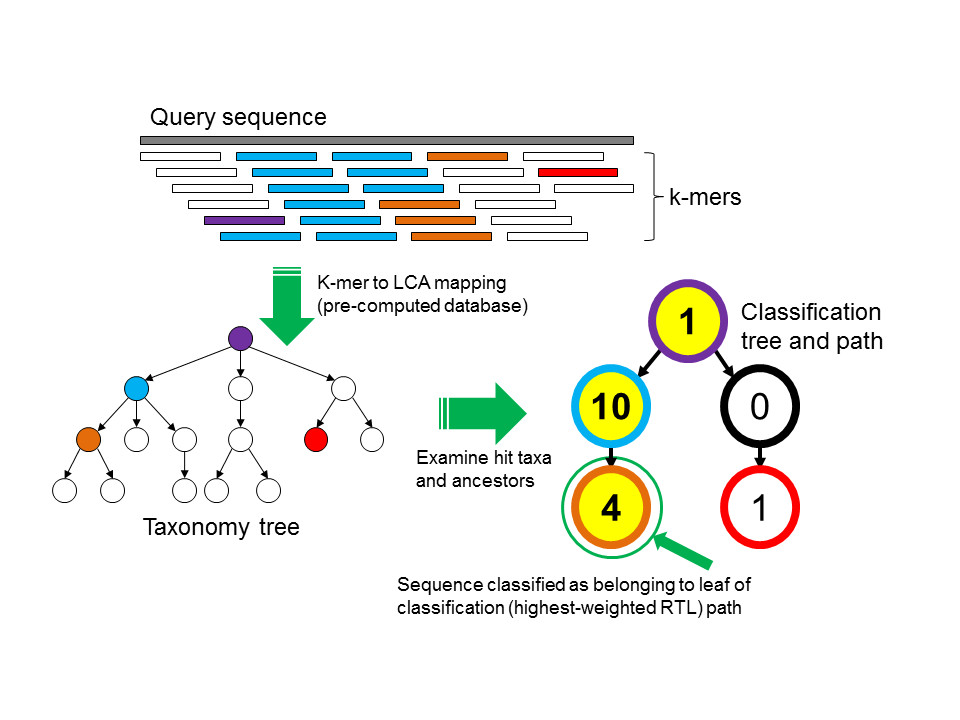
\includegraphics[width=\textwidth]{Work.jpg}
	\caption{Prikaza klasifikacije podataka}
	\label{Klasifikacija}
\end{figure}


\newpage
\subsection{LCA(\textit{Lower Common Ancestor})}
%TODO ubacit sliku za LCA
LCA(\textit{Lower common ancestor}) je jedan od osnovnih algoritamskih problema u strukturama stabala. Prvu ideju i definiciju LCA dali su Alfred Aho, John Hopcroft i Jeffrey Ullman 1973. godine u svom radu \textit{On finding lowest common ancestors in trees}. Problem se odnosi na to da se za dva cvora \textit{x} i \textit{y} nađe najbliži čvor u stablu koji je hijerarhijom viši, te je zajedniči oba čvora. Ovaj problem je važan ne samo zbog svoje složenosti i razumjevanja strukture stabala, nego i zbog svoje primjene. Jedna od primjena je u bioinformatici za određivanje zajedničkog pretka dvije različite vrste. Upravo Kraken koristi LCA kao metodu određivanja navedenog iz k-mera podataka.
\chapter{Algoritmi indeksiranja i pretrage}
\subsection{Minimizer - algoritam za reduciranje podataka}
S obzirom na veličinu podataka koji se koriste u metagenomici nailazilo se na problem spremanja istih u RAM. Na ideju rješenja su došli Michael Roberts, Wayne Hayes, Brian R. Hunt, Stephen M. Mount i James A. York u svom radu \textit{Reducing storage requirements for biological sequence comparison}. Način rada se bazira na tome da se radi \textit{seed-and-extend}. Od ulaznog niz se uzimaju određeni dijelovi koji karakteriziraju dani niz, te se poravnava sa karakterističnim podnizovima drugog niza. Kada se uspiju poravnat string se proširuje i traže se druga poravnanja. Ovo uvelika smanjuje bazu podataka koju Kraken koristi, zbog toga što se u kontejnerima koje sadrže podatke istih k-mera nalaze samo vrijednosti podnizova koje se poslije dinamično proširuju.\\Nakon poravnanja i sažimanja podataka oni moraju zadovoljavaju kriterij kolekcije, tj moraju koliko toliko zadovoljavati normalnu razdiobu u kontejnere. Stoga je potrebno osposobit taj način rada tako da dva slična niza biraju svoje k-mere na način da će se lako naći poravnanje , te  s tim uspjeti usporediti pravilno. \\Minimizer algoritam radi tako da se niz sortira leksikografski te se iz toga biraju minimizer vrijednosti. Prvo se izvedu sve moguće k-mere, te se niz poreda leksikografski, tada se od danih k-mera odabiru one najmanje. Ako postoji više najmanjih k-mera, tada su sve one minimizer vrijednosti.
%TODO ubaciti sliku određivana minimizer vrijednosti.


\subsection{Binarno pretraživanje}
\chapter{Pseudokod i razrada algoritma}
\chapter{Analiza učinkovitosti rješenja}
\chapter{Zaključak}
Zaključak.

\bibliography{literatura}
\bibliographystyle{fer}

\begin{sazetak}
Sažetak na hrvatskom jeziku.

\kljucnerijeci{Ključne riječi, odvojene zarezima.}
\end{sazetak}

% TODO: Navedite naslov na engleskom jeziku.
\engtitle{Title}
\begin{abstract}
Abstract.

\keywords{Keywords.}
\end{abstract}

\end{document}
